\newif\ifglobal

%%%%%%%%%%%%%%%%%%%%%%%
%%% Compile to view %%%
%%%%%%%%%%%%%%%%%%%%%%%

%%%%%%%%%%%%%%%%%%%%%%%%%%%%%%%%%%%%%%%%%%%%%%%%%%%
%%% Readme:                                     %%%
%%% https://www.overleaf.com/read/bwdjvfjksvjy/ %%%
%%%%%%%%%%%%%%%%%%%%%%%%%%%%%%%%%%%%%%%%%%%%%%%%%%%

% >>> M?: marks a module setting number or important notice

% >>> M4: Set {./relative-path} to external files for this module <<<
\def \modulefiles {./23-PCNT}
% To add an external file, use:
% (Replace '---' with actual filename)
% '\input{\modulefiles/tables/---.tex}' for tables
% '\includegraphics{\modulefiles/figures/---}' for figures
% '\subfile{\modulefiles/---}' for register files

% >>> M1: This module is in global project? <<<
% 'YES' - uncomment; 'NO' - comment out
\globaltrue

\ifglobal
    \documentclass[main\_\_EN.tex]{subfiles}

\else
    \documentclass[openany, 10pt]{book}

    % >>> M2: In ./00-shared/preamble-trm-module, also find
    %         settings for visibility of todo notes, watermark <<<
    \usepackage{preamble-trm-module}

    % >>> M3: Temporary labels in English,
    %         you can add your own labels there <<<
    \myexternaldocument{./00-shared/temp-labels-en}

\fi %\ifglobal


\setcounter{secnumdepth}{4}


% >>> M5: If this module needs any updates in
% './00-shared/preamble-trm-module.sty'
% (include additional package, etc.), contact your module PM
% or create the file './00-shared/changelog.tex' make the
% necessary updates yourself and document them in this file <<<

% Make text left-aligned and allow latex to break pages naturally, comment out for full justification
\raggedright
\raggedbottom


\begin{document}


% Sets language into which pre-defined bits of text are translated
\selectlanguage{english}
\setenglishformatting

% Do not delete this block
\ifglobal
% Add the following front matter if
% this module is outside of global project
\else
    \InputIfFileExists{readme}{}{}
    \listoftodos
    {\let\clearpage\relax \listofdonetodos}
    \tableofcontents
    %\listoftables
    %\listoffigures
\fi


%%%%%%%%%%%%%%%%%%%%%%%%%
%%% TRM Module Begins %%%
%%%%%%%%%%%%%%%%%%%%%%%%%

\hypertarget{pcnt}{}
\chapter{Pulse Count Controller (PCNT)}
\label{mod:pcnt}

\section{Overview}
The pulse counter module is designed to count the number of rising and/or falling edges of an input signal. Each pulse counter unit has a 16-bit signed counter register and two channels that can be configured to either increment or decrement the counter. Each channel has a signal input that accepts signal edges to be detected, as well as a control input that can be used to enable or disable the signal input. The inputs have optional filters that can be used to discard unwanted glitches in the signal.

The pulse counter has eight independent units, referred to as PULSE\_CNT\_U\textcolor{red}{\it{n}}.

The maximum frequency of pulses supported by ESP32's pulse counter is 40 MHz.

\section{Functional Description}

\subsection{Architecture}

\begin{figure}[H]
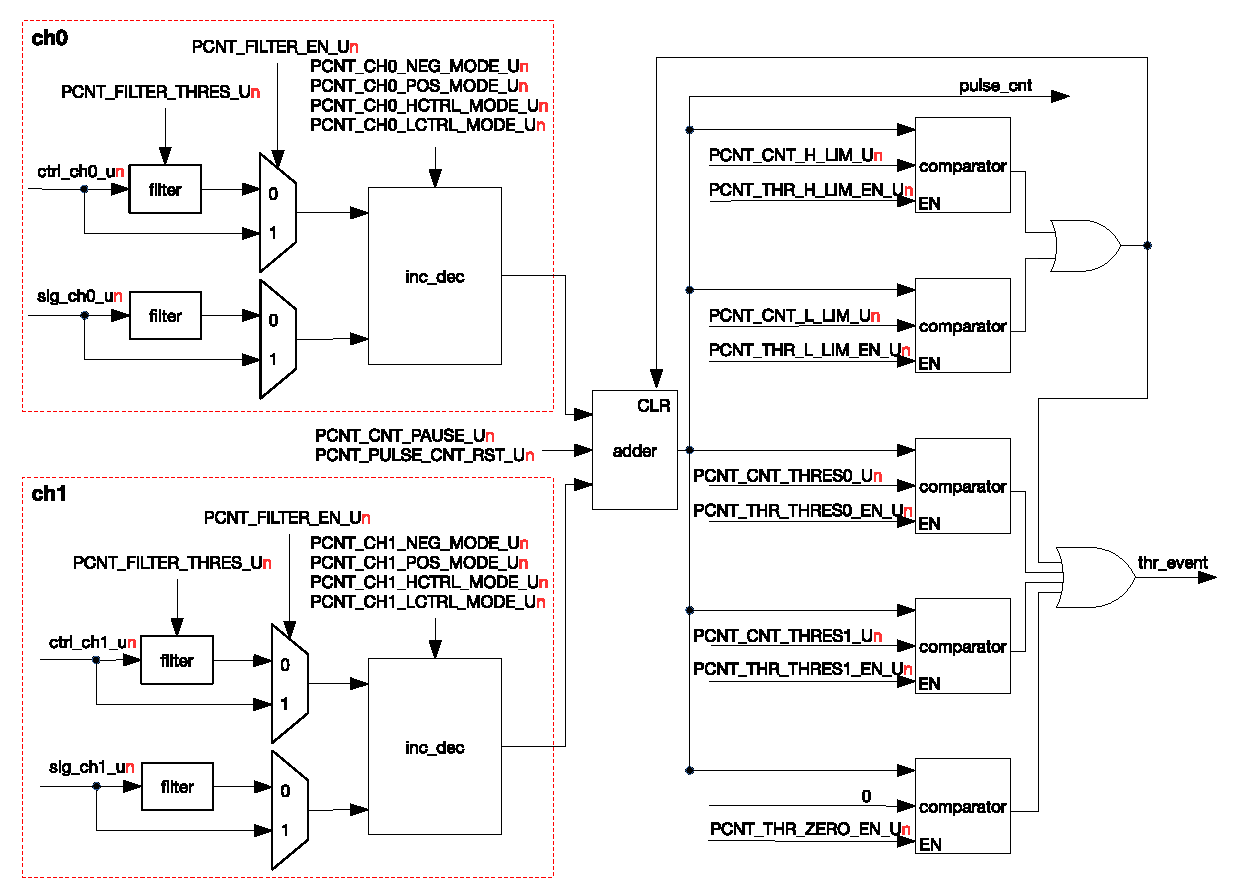
\includegraphics[width=1\textwidth]{./23-PCNT/figures/pcnt_arch_updated}
\centering
\caption{PULSE\_CNT Architecture}
\label{Figure:pulse_cnt_architecture}
\end{figure}

The architecture of a pulse counter unit is illustrated in Figure \ref{Figure:pulse_cnt_architecture}. Each unit has two channels: ch0 and ch1, which are functionally equivalent. Each channel has a signal input, as well as a control input, which can both be connected to I/O pads. The counting behavior on both the positive and negative edge can be configured separately to increase, decrease, or do nothing to the counter value. Separately, for both control signal levels, the hardware can be configured to modify the edge action: invert it, disable it, or do nothing. The counter itself is a 16-bit signed up/down counter. Its value can be read by software directly, but is also monitored by a set of comparators which can trigger an interrupt.

\subsection{Counter Channel Inputs}
As stated before, the two inputs of a channel can affect the pulse counter in various ways. The specifics of this behaviour are set by LCTRL\_MODE and HCTRL\_MODE in this case when the control signal is low or high, respectively, and POS\_MODE and NEG\_MODE for positive and negative edges of the input signal. Setting POS\_MODE and NEG\_MODE to 1 will increase the counter when an edge is detected, setting them to 2 will decrease the counter and setting at any other value will neutralize the effect of the edge on the counter. LCTR\_MODE and HCTR\_MODE modify this behaviour, when the control input has the corresponding low or high value: 0 does not modify the NEG\_MODE and POS\_MODE behaviour, 1 inverts it (setting POS\_MODE/NEG\_MODE to increase the counter should now decrease the counter and vice versa) and any other value disables counter effects for that signal level.

To summarize, a few examples have been considered. In this table, the effect on the counter for a rising edge is shown for both a low and a high control signal, as well as various other configuration options. For clarity, a short description in brackets is added after the values. Note: x denotes 'do not care'.

\begin{longtable}{ | p{3cm} | p{3cm} | p{3cm} | p{3cm} | p{3cm} |  } \hline
\rowcolor{lightgray}
POS\_ MODE & LCTRL\_ MODE & HCTRL\_ MODE  & sig l$\rightarrow$h when ctrl=0 & sig l$\rightarrow$h when ctrl=1 \\ \hline
1 (inc) & 0 (-) & 0 (-) & Inc ctr & Inc ctr \\ \hline
2 (dec) & 0 (-) & 0 (-) & Dec ctr & Dec ctr \\ \hline
0 (-) & x & x & No action & No action \\ \hline
1 (inc) & 0 (-) & 1 (inv) & Inc ctr & Dec ctr \\ \hline
1 (inc) & 1 (inv) & 0 (-) & Dec ctr & Inc ctr \\ \hline
2 (dec) & 0 (-) & 1 (inv) & Dec ctr & Inc ctr \\ \hline
1 (inc) & 0 (-) & 2 (dis) & Inc ctr & No action \\ \hline
1 (inc) & 2 (dis) & 0 (-) & No action & Inc ctr \\ \hline
\end{longtable}

This table is also valid for negative edges (sig h$\rightarrow$l) on substituting NEG\_MODE for POS\_MODE.

Each pulse counter unit also features a filter on each of the four inputs, adding the option to ignore short glitches in the signals. If a PCNT\_FILTER\_EN\_U\textcolor{red}{\it{n}} can be set to filter the four input signals of the unit. If this filter is enabled, any pulses shorter than REG\_FILTER\_THRES\_U\textcolor{red}{\it{n}} number of APB\_CLK clock cycles will be filtered out and will have no effect on the counter. With the filter disabled, in theory infinitely small glitches could possibly trigger pulse counter action. However, in practice the signal inputs are sampled on APB\_CLK edges and even with the filter disabled, pulse widths lasting shorter than one APB\_CLK cycle may be missed.

Apart from the input channels, software also has some control over the counter. In particular, the counter value can be frozen to the current value by configuring PCNT\_CNT\_PAUSE\_U\textcolor{red}{\it{n}}. It can also be reset to 0 by configuring PCNT\_PLUS\_CNT\_RST\_U\textcolor{red}{\it{n}}.

\subsection{Watchpoints}\label{Watchpoints}

The pulse counters have five watchpoints that share one interrupt. Interrupt generation can be enabled or disabled for each individual watchpoint. The watchpoints are:

\begin{itemize}
    \item Maximum count value: Triggered when PULSE\_CNT >= PCNT\_CNT\_H\_LIM\_U\textcolor{red}{\it{n}}. Additionally, this will reset the counter to 0. PCNT\_CNT\_H\_LIM\_U\textcolor{red}{\it{n}} should be a positive number.
    \item Minimum count value: Triggered when PULSE\_CNT <= PCNT\_CNT\_L\_LIM\_U\textcolor{red}{\it{n}}. Additionally, this will reset the counter to 0. PCNT\_CNT\_L\_LIM\_U\textcolor{red}{\it{n}} should be a negative number.
    \item Two threshold values: Triggered when PULSE\_CNT = PCNT\_THR\_THRES0\_U\textcolor{red}{\it{n}} or PCNT\_THR\_THRES1\_U\textcolor{red}{\it{n}}.
    \item Zero: Triggered when PULSE\_CNT = 0.
\end{itemize}

\subsection{Examples}

\begin{figure}[H]
\fbox{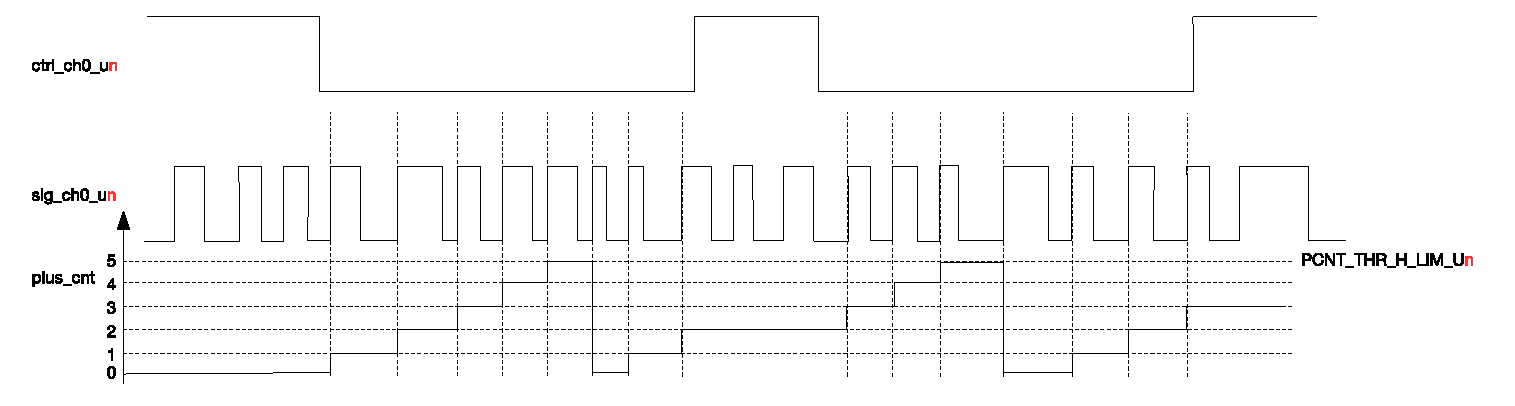
\includegraphics[width=0.7\textwidth]{./23-PCNT/figures/pulse_add}}
\centering
\caption{PULSE\_CNT Upcounting Diagram}
\label{Figure:pulse_add}
\end{figure}

Figure \ref{Figure:pulse_add} shows channel 0 being used as an up-counter. The configuration of channel 0 is shown below.

\begin{itemize}
    \item CNT\_CH0\_POS\_MODE\_U\textcolor{red}{\it{n}} = 1: increase counter on the rising edge of sig\_ch0\_u\textcolor{red}{\it{n}}.
    \item PCNT\_CH0\_NEG\_MODE\_U\textcolor{red}{\it{n}} = 0: no counting on the falling edge of  sig\_ch0\_u\textcolor{red}{\it{n}}.
    \item PCNT\_CH0\_LCTRL\_MODE\_U\textcolor{red}{\it{n}} = 0: Do not modify counter mode when ctrl\_ch0\_u\textcolor{red}{\it{n}} is low.
    \item PCNT\_CH0\_HCTRL\_MODE\_U\textcolor{red}{\it{n}} = 2: Do not allow counter increments/decrements when ctrl\_ch0\_u\textcolor{red}{\it{n}} is high.
    \item PCNT\_CNT\_H\_LIM\_U\textcolor{red}{\it{n}} = 5: PULSE\_CNT resets to 0 when the count value increases to 5.
\end{itemize}

\begin{figure}[H]
\fbox{
\includegraphics[width=0.7\textwidth]{./23-PCNT/figures/pulse_dec}}
\centering
\caption{PULSE\_CNT Downcounting Diagram}
\label{Figure:pulse_dec}
\end{figure}

Figure \ref{Figure:pulse_dec} shows channel 0 decrementing the counter. The configuration of channel 0 differs from that in Figure \ref{Figure:pulse_add} in the following two aspects:

\begin{itemize}
    \item PCNT\_CH0\_LCTRL\_MODE\_U\textcolor{red}{\it{n}} = 1: invert counter mode when ctrl\_ch0\_u\textcolor{red}{\it{n}} is at low level, so it will decrease, rather than increase, the counter.
    \item PCNT\_CNT\_H\_LIM\_U\textcolor{red}{\it{n}} = –5: PULSE\_CNT resets to 0 when the count value decreases to –5.
\end{itemize}

\subsection{Interrupts}

\label{int:PCNTCNTTHREVENTUnINT}PCNT\_CNT\_THR\_EVENT\_U\textcolor{red}{\it{n}}\_INT: This interrupt gets triggered when one of the five channel comparators detects a match.

\hypertarget{pcnt-reg-summ}{}
\section{Register Summary}\label{sec:pcnt-reg-summ}

The addresses in this section are relative to the PCNT base address provided in Table \ref{table:Peripheral_Address_Mapping} in Chapter \ref{mod:sysmem} \textit{\nameref{mod:sysmem}}.

The abbreviations given in Column \textbf{Access} are explained in Section \hyperref[glossary-access-types]{\textit{Access Types for Registers}}.


\subfile{\modulefiles/pulsecnt_reg_summary_en.tex}

\section{Registers}

The addresses in this section are relative to the PCNT base address provided in Table \ref{table:Peripheral_Address_Mapping} in Chapter \ref{mod:sysmem} \textit{\nameref{mod:sysmem}}. The absolute register addresses are listed in Section \ref{sec:pcnt-reg-summ} \textit{\nameref{sec:pcnt-reg-summ}}. 

For how to program reserved fields, please refer to Section \hyperref[programming-reserved-field]{\textit{Programming Reserved Register Field}}.


\subfile{\modulefiles/pulsecnt_reg_en.tex}


\end{document}
